\documentclass[xcolor=table]{beamer}

\usepackage{booktabs}
\usepackage{hyperref}
\usepackage[table]{xcolor}
\usepackage{tikz}

\setbeamertemplate{navigation symbols}{}%remove navigation symbols

\title{Next generation consoles and an introduction to extensive form games}
\subtitle{Game Theory}
\author{Vincent Knight}
\date{}

\tikzstyle{level 1}=[level distance=3.5cm, sibling distance=3.5cm]
\tikzstyle{level 2}=[level distance=3.5cm, sibling distance=2cm]
\tikzstyle{player} = [text width=4em, draw, text centered, rectangle, fill=blue!20, inner sep=1pt]
\tikzstyle{nature} = [minimum width=3pt,circle,  draw, fill=red!20, inner sep=1pt]
\tikzstyle{end} = [circle, minimum width=3pt, fill, inner sep=0pt, right]

\begin{document}

\frame{\titlepage}

\frame{Elliot and I want to get a next gen games console:
\vspace{1cm}
\begin{center}
\begin{tikzpicture}
\node at (0,0) [red]{Xbox One};
\node (PS4) at (4,0) [blue] {PS4};
\pause
\node (C) at (2,-2) {We both prefer};
\draw (C) edge[out=0, in=-90, ->] (PS4);
\pause
\node at (5,1) [draw, blue, circle] {$90\%$};
\end{tikzpicture}
\end{center}
}

\frame{
\begin{center}
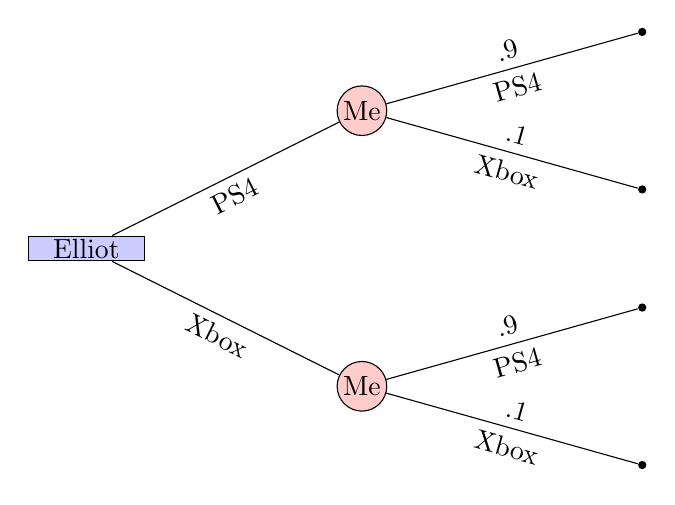
\begin{tikzpicture}[grow=right, sloped]
    \node[player]{Elliot}
        child {node[nature] {Me}
                child {node[end] {} edge from parent node[above] {.1} node[below] {Xbox}}
                child {node[end] {} edge from parent node[above] {.9} node[below] {PS4}} edge from parent node[below] {Xbox}}
        child {node[nature] {Me}
                child {node[end] {} edge from parent node[above] {.1} node[below] {Xbox}}
                child {node[end] {} edge from parent node[above] {.9} node[below] {PS4}} edge from parent node[below] {PS4}};
\end{tikzpicture}
\end{center}
}

\frame{
\begin{itemize}
\item A finite set of $N$ players: Elliot and I.
\item A rooted tree.
\item An $N-tuple$ of payoffs: `how happy we will be at each leaf of the tree'
\end{itemize}
}

\frame{
\begin{center}
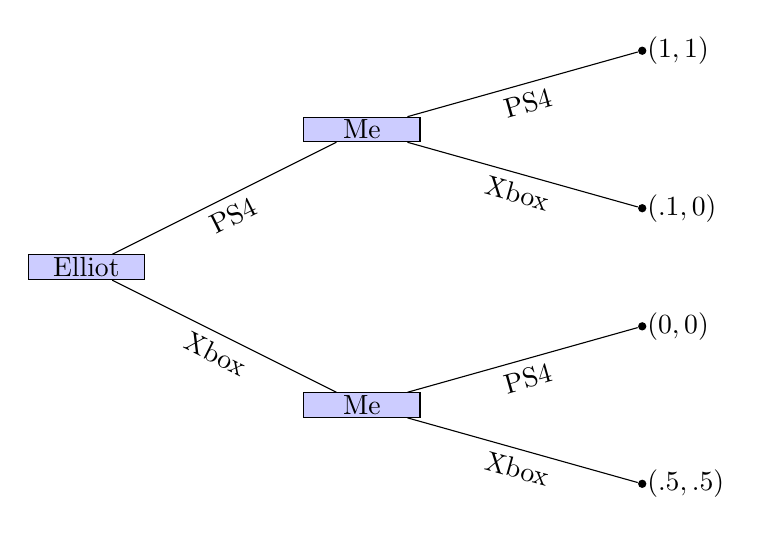
\begin{tikzpicture}[grow=right, sloped]
    \node[player]{Elliot}
        child {node[player] {Me}
                child {node[end] {} node[right] {$(.5,.5)$} edge from parent node[below] {Xbox}}
                child {node[end] {} node[right] {$(0,0)$} edge from parent node[below] {PS4}} edge from parent node[below] {Xbox}}
        child {node[player] {Me}
                child {node[end] {} node[right] {$(.1,0)$} edge from parent node[below] {Xbox}}
                child {node[end] {} node[right] {$(1,1)$} edge from parent node[below] {PS4}} edge from parent node[below] {PS4}};
\end{tikzpicture}
\end{center}}

\frame{
\begin{center}
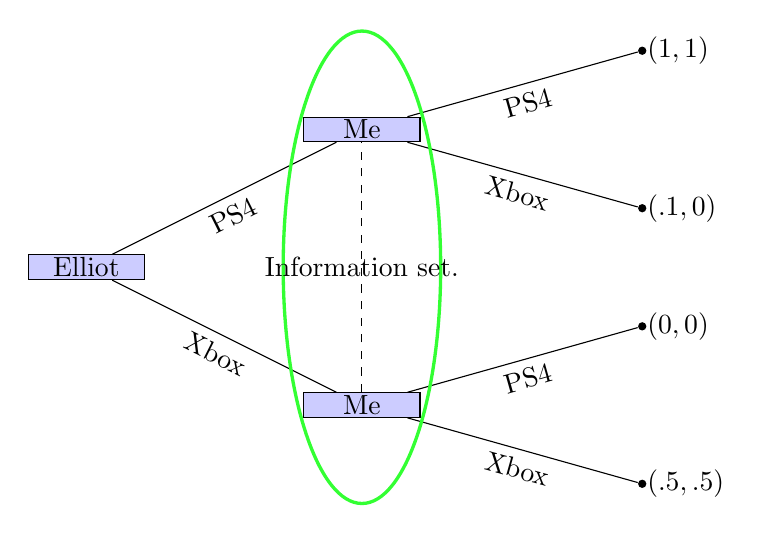
\begin{tikzpicture}[grow=right, sloped]
    \node[player]{Elliot}
        child {node[player] (b) {Me}
                child {node[end] {} node[right] {$(.5,.5)$} edge from parent node[below] {Xbox}}
                child {node[end] {} node[right] {$(0,0)$} edge from parent node[below] {PS4}} edge from parent node[below] {Xbox}}
        child {node[player] (c) {Me}
                child {node[end] {} node[right] {$(.1,0)$} edge from parent node[below] {Xbox}}
                child {node[end] {} node[right] {$(1,1)$} edge from parent node[below] {PS4}} edge from parent node[below] {PS4}};
    \draw[dashed] (b) -- (c);
    \pause
    \draw [color=green!80, very thick] (3.5,0) ellipse  (1 and 3);
    \node at (3.5,0) {Information set.};
\end{tikzpicture}
\end{center}

}

\end{document}
